\noindent
\begin{tabular}{cc}
\begin{minipage}[l]{0.50\textwidth}
 \begin{exerciseS}[Corrente di Poiseuille in un canale piano e manometro]
 Una corrente di Poiseuille di acqua ($\rho = 1000 / kg/m^3$, $\mu = 
 10^{-3} \ kg/(m s)$) scorre in 
 un canale di altezza $H = 1 \ cm$. Un manometro misura la differenza di 
 pressione tra le sezioni in $x_A = 1.0 \ m$ e $x_B= 2.0 \ m$.
 Determinare:
 \begin{itemize}
   \item il gradiente di pressione all'interno del condotto, conoscendo la
       densità del liquido barometrico $\bar{\rho} = 1200 \ kg/m^3$ e la 
       differenza di quote $h = 5 \ mm$;
   \item la velocità massima all'interno del canale;
   \item la risultante $\bm{R}$ delle forze esercitata dal fluido sul tratto
      di parete superiore compreso tra A e B, sapendo che sulla sezione
      $x = 0 \ m$ la pressione vale $p_0 = 10^5 \ Pa$. Qual è la relazione
      tra $R_x$ e $p_A - p_B$? Commento.
 \end{itemize}
 \end{exerciseS}
\end{minipage}
\hspace{3mm}
\begin{minipage}[r]{0.50\textwidth}
   \begin{center}
   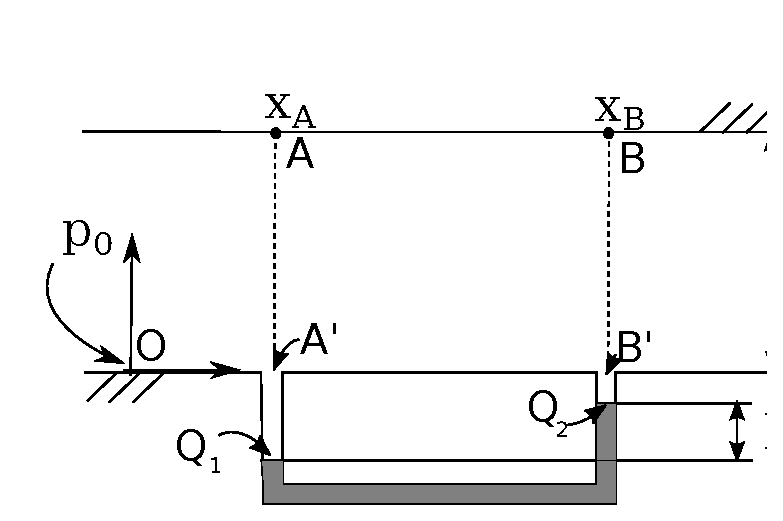
\includegraphics[width=0.90\textwidth]{./fig/manometro_Poiseuille.eps}
   \end{center}
\end{minipage}
\end{tabular}

\sol

\partone Soluzione esatte delle equazioni di Navier-Stokes. Corrente di
 Poiseuille nel canale piano 2D. Manometro: leggi della statica (Stevino).

\parttwo
\begin{itemize}
\item
Per trovare la derivata in direzione $x$ della pressione all'interno del
 canale ($\partial P/\partial x = - G_P = cost.$ per la corrente di Poiseuille) risolve il problema di statica all'interno del manometro.
Facendo riferimento al disegno, si utilizza Stevino tra i punti $A'-Q_1$,
 $Q_1-Q_2$, $Q_2-B'$ e l'informazione di derivata della pressione costante
 in direzione $x$ all'interno del canale, tra $A'$ e $B'$.
\begin{equation}
 \begin{cases}
  p_{A'} = p_{Q_1} - \rho g z_{Q_1} \\
  p_{Q_1} - \bar{\rho} g z_{Q_1} =   p_{Q_2} - \bar{\rho} g z_{Q_2} \\
  p_{B'} = p_{Q_2} - \rho g z_{Q_2} \\
  p_{A'} - p_{B'} = G_P \Delta x
 \end{cases} \Rightarrow
  G_P = \dfrac{1}{\Delta x}(\bar{\rho}-\rho) g \Delta h
\end{equation}
avendo svolto correttamente i conti e riconosciuto $z_{Q_2} - z_{Q_1} =
 \Delta h$.

\item
Ricordando che il profilo di velocità di Poiseuille risulta
 $\bm{u} = \bm{\hat{x}} u(y)$, con 
\begin{equation}
 u(y) = -\dfrac{G_P}{2 \mu} y (y-H),
\end{equation}
 la velocità massima all'interno del canale è $V = u(H/2) =
 \dfrac{G_P}{8 \mu} H^2$

\item
Per calcolare la risultante degli sforzi sul tratto $A-B$ della parete 
 superiore, è necessario calcolare il vettore sforzo agente su di essa
 e svolgere un semplice integrale.
Il vettore sforzo agente sulla parete superiore risulta
 \begin{equation}
  \bm{t} = - \mu \dfrac{\partial u}{\partial y}\bigg|_{y=H} \bm{\hat{x}} +
           p(x,H) \bm{\hat{y}} \ .
 \end{equation}
 La pressione $p(x,H)$ sulla parete superiore, per $x \in [x_A,x_B]$ si
 calcola come segue: si parte dall'origine del sistema di riferimento $O$,
 in corrispondenza della quale è noto il valore della pressione $p_0$ e ci 
 si muove in orizzontale ricordando che $\partial P/\partial x = -G_P$ e
 in verticale ricordando che $\partial P/\partial y = -\rho g$.
 \begin{equation}
 \begin{aligned}
  p_{A'} & = p_0 - G_P x_A \\
  p_{A } & = p_{A'} - \rho g H  \\
%  p_{B } & = p_{A}  - G_P (x_B - x_A)  \\ \\
 \end{aligned}
 \qquad \rightarrow  \qquad p(x,H)  = p_{A} - G_P ( x  -x_A )
 \end{equation}
 Lo sforzo tangenziale sulla parete è costante e vale
 \begin{equation}
  - \mu \dfrac{\partial u}{\partial y}\bigg|_{y=H} =
    \dfrac{G_P}{2} H
 \end{equation}
 La risultante delle forze (per unità di lunghezza, poichè il problema
  è bidimensionale) si ottiene integrando lo sforzo tra $A$ e $B$. Facendo comparire il valore $p_B$ della pressione in $B$, l'espressione della risultante delle forze diventa
 \begin{equation}
  \bm{R} = \dfrac{G_P}{2} H \Delta x \bm{\hat{x}} + 
           \dfrac{1}{2}(p_A + p_B) \Delta x \bm{\hat{y}} \ .
 \end{equation}


\end{itemize}
